%% Преамбула TeX-файла

% 1. Стиль и язык
\documentclass[utf8x, 13pt]{G7-32}
\usepackage{float}

% Остальные стандартные настройки убраны в preamble.inc.tex.
\sloppy

% Настройки стиля ГОСТ 7-32
% Для начала определяем, хотим мы или нет, чтобы рисунки и таблицы нумеровались в пределах раздела, или нам нужна сквозная нумерация.
\EqInChapter % формулы будут нумероваться в пределах раздела
\TableInChapter % таблицы будут нумероваться в пределах раздела
\PicInChapter % рисунки будут нумероваться в пределах раздела

% Добавляем гипертекстовое оглавление в PDF
\usepackage[
bookmarks=true, colorlinks=true, unicode=true,
urlcolor=black,linkcolor=black, anchorcolor=black,
citecolor=black, menucolor=black, filecolor=black,
]{hyperref}

% Изменение начертания шрифта --- после чего выглядит таймсоподобно.
% apt-get install scalable-cyrfonts-tex

\IfFileExists{cyrtimes.sty}
    {
        \usepackage{cyrtimespatched}
    }
    {
        % А если Times нету, то будет CM...
    }

\usepackage{graphicx}   % Пакет для включения рисунков

% С такими оно полями оно работает по-умолчанию:
% \RequirePackage[left=20mm,right=10mm,top=20mm,bottom=20mm,headsep=0pt]{geometry}
% Если вас тошнит от поля в 10мм --- увеличивайте до 20-ти, ну и про переплёт не забывайте:
\geometry{right=15mm}
\geometry{left=30mm}
\geometry{top=20mm}
\geometry{bottom=15mm}

% Пакет Tikz
\usepackage{tikz}
\usetikzlibrary{shapes,arrows,positioning,shadows}
\tikzset{
  main/.style={circle, minimum size = 30mm, thick, draw =black!80, node distance = 10mm},
  connect/.style={-latex, thick},
  box/.style={rectangle, draw=black!100}
}

% Произвольная нумерация списков.
\usepackage{enumerate}

% ячейки в несколько строчек
\usepackage{multirow}

% itemize внутри tabular
\usepackage{paralist,array}

% Центрирование подписей к плавающим окружениям
\usepackage[justification=centering]{caption}

% для ссылки на последнюю страницу
\usepackage{lastpage}


% Настройки листингов.
\ifPDFTeX
\include{listings.inc}
\else
\usepackage{local-minted}
\fi

% Полезные макросы листингов.
% Любимые команды
\newcommand{\todo}[1]{\Large{\textcolor{red}{#1}}\normalsize}
\newcommand{\Code}[1]{\textbf{#1}}


\begin{document}

\frontmatter % выключает нумерацию ВСЕГО; здесь начинаются ненумерованные главы: реферат, введение, глоссарий, сокращения и прочее.

\newpage

\begin{center}
{\small \textbf{Федеральное государственное автономное образовательное учреждение высшего образования
«Национальный исследовательский университет «Московский институт электронной техники»}}
\end{center}

\begin{flushleft}
{\small \textbf{Факультет} \underline{микроприборов и технической кибернетики}} \linebreak
{\small \textbf{Кафедра} \underline{информатики и программного обеспечения вычислительных систем}}
\end{flushleft}

\vspace{1em}

\begin{center}
\textsc{\textbf{Магистерская диссертация}}
\end{center}

\begin{center}
\textbf{на тему:}
\end{center}

\vspace{1.0em}

\begin{center}
Исследование и разработка методики и алгоритма обработки и~структуризации библиографических данных
\end{center}

\vspace{1em}

\begin{center}
на соискание степени магистра по направлению подготовки \linebreak
09.04.04 “Программная инженерия”
\end{center}

\begin{center}
Программа “Программное обеспечение автоматизированных систем и \linebreak
вычислительных комплексов”
\end{center}

\vspace{\fill}

\begin{flushright}
\textbf{Научный руководитель} доц., к.т.н \linebreak
Кононова А.И. \linebreak
\rule{5cm}{.1pt}

\vspace{1em}

\textbf{Магистрант} ИПОВС-12 \linebreak
Петров Е.Н. \linebreak
\rule{5cm}{.1pt}
\end{flushright}

\begin{center}
Москва 2017 г.
\end{center}

\thispagestyle{empty}

\tableofcontents

%\include{10-defines}

\Introduction
 
В настоящее время в вузах существует практика сбора сведений о публикациях преподавательского состава и студентов кафедр. Эти сведения подаются преподавателями коллективно или в индивидуальном порядке ответственному лицу, которое на основе полученных данных формирует единый отчет в виде, требуемом отделом научно-технической информации.

Формирование отчета представляет собой рутинный труд по переносу предоставленных данных в сводную таблицу, отвечающую заявленным требованиям. Как и во всякой рутинной работе, выполняемой вручную, велико влияние человеческого фактора на результат, будь то опечатки, в том числе вставка информации не в ту ячейку, или пропущенные по неосторожности публикации. Описанные ошибки ответственного лица существенно снижают эффективность и качество работы, а обнаружение этих ошибок не всегда является простой задачей.

Помимо этого, требования к оформлению итогового отчета могут изменяться, поэтому не всегда очевидно, какая информация может пригодиться, а какая - нет. В зависимости от характера изменений, необходимо будет переделать один или несколько столбцов сводной таблицы, вручную переформатировать некоторые ячейки, добавить или удалить определенную информацию. При большом количестве исходных данных любое изменение в требованиях к итоговому отчету может обернуться трудо- и времязатратными  исправлениями.

Очевидно, что ручная обработка большого объема библиографических данных является неэффективной как по времени, так и по качеству; с другой стороны, выполнение данной работы компьютером гарантирует отсутствие ошибок по невнимательности, универсальность обработки различных форматов данных, структуризацию и быстроту обработки и, как следствие, своевременную отчетность.

Таким образом, \textbf{является актуальной} задача выполнения процесса обработки и структуризации библиографических данных с помощью компьютера, которая заключается в переводе этих данных из различных форматов в единое представление.
 
Существующие информационные системы, использующие алгоритмы обработки библиографических данных, предполагают либо строгое соответствие данных определенным стандартам, таким как ГОСТ 5.0.7 - 2008, MARC и другим, что на практике труднодостижимо, так как речь идет не о переводе из одного формата в другой, а о переносе подаваемых преподавательским составом в независимое представление; либо используют современные технологии в сочетании с англоязычными словарями, что, пусть и исключает привязку к определенному формату, существенно влияет на качество работы с русскоязычными библиографическими сведениями в целом и со сведениями, оформленными в соответствии с ГОСТ 5.0.7 - 2008 в частности.

Поэтому было принято решение о разработке собственного алгоритма, в полной мере поддерживающего русский язык и способного проявлять гибкость при обработке и не следовать определенному формату.

\textbf{Объектом исследования} являются библиографические данные.

\textbf{Предметом исследования} из всей области научных изысканий, представляющих объект исследования, были выбраны обработка и структуризация библиографических данных.

\textbf{Цель работы} заключается в исследовании и разработке нового алгоритма и методики обработки и структуризации библиографических данных, обеспечивающих поддержку русского языка и корректную обработку отступлений от определенного формата.

\textbf{Задачами исследования} являются:
\begin{itemize}
	\item обзор современного состояния информационных систем для обработки и структуризации библиографических данных;
	\item исследование методов обработки и структуризации библиографических данных в информационных системах;
	\item исследование и разработка методики и алгоритма обработки и структуризации библиографических данных;
	\item разработка и программная реализация программного средства, реализующего разработанный алгоритм.
\end{itemize}

В диссертации в качестве \textbf{методов исследования} используются методы теории автоматов, методы построения нейронных сетей, статистические методы и методы машинного обучения.

\textbf{Научная новизна исследования} состоит в создании новых методики и алгоритма обработки и структуризации библиографических данных.

Были исследованы современные методы обработки и структуризации библиографических данных. На основе этого анализа был выбран метод условно-случайных полей, наиболее подходящий для решения проблемы компьютеризации процесса обработки и структуризации библиографических данных.

Выбранный метод условно-случайных полей был применен к задаче обработки и структуризации библиографических данных на русском языке, оформленных в разной степени соответствия стандарту ГОСТ 5.0.7 - 2008, наиболее распространенному в нашей стране.

Для проверки работы метода был выбран набор меток, отражающих различные структурные элементы, составлена графовая модель состояний и переходов, а также проведена работа по выделению ключевых признаков структурных элементов и составлению их функций.

Среди ключевых функций признаков были выделены следующие группы: функции положения слова в предложении, функции символьного состава слова, регистровые функции и функции совпадения со служебными символами стандарта ГОСТ 5.0.7 - 2008. Ряд функций признаков был отброшен в процессе исследования, так как отрицательно сказывался на точности работы метода.

На основе полученных результатов были сформированы методика и алгоритм обработки и структуризации библиографических данных, а также было разработано программное средство обработки и структуризации библиографических данных, реализующее метод условно-случайных полей в соответствии с разработанной графовой моделью состояний и переходов и выделенными функциями признаков.

\textbf{Практическая значимость результатов} исследования заключается в обеспечении эффективного управления библиографическими сведениями вузов и других образовательных и научных учреждений, библиотек, научно-исследовательских и прочих организаций, работающих с библиографическими данными, за счет замены ручной обработки данных на компьютерную, осуществляемую на основе разработанных методики и алгоритма.

Результаты исследования позволят выполнять обработку и структуризацию библиографических данных на русском языке без использования явно заданного формата, опираясь только на признаки отдельных структурных компонентов библиографической записи, а не на их последовательность или структуру записи в целом.

Такой подход к обработке позволит осуществлять перевод библиографических данных из одного представления или формата в другой с минимальным участием оператора, в том числе исправлять ошибки форматирования и следования структурных компонентов в рамках одного стандарта оформления.

\textbf{Структура диссертации} состоит из введения, четырех глав, заключения, списка литературы и приложений. Работы содержит \_ страниц основного текста, \_ страниц с рисунками и таблицами, список литературы из \_ наименований, \_ приложения на \_ страницах.

\textbf{На защиту выносятся} следующие положения и результаты:
\begin{itemize}
	\item выявлены требования к информационной системе для обработки и структуризации библиографических данных;
	\item выделены структурные элементы, достаточные для решения задачи структуризации библиографических данных;
	\item выявлены ключевые признаки структурных элементов и составлены их функции;
	\item разработаны методика и алгоритм обработки и структуризации библиографических данных.
\end{itemize}


\mainmatter % это включает нумерацию глав и секций в документе ниже

\chapter{Современное состояние программных средств и алгоритмов классификации библиографических данных}

В настоящее время обработка библиографических данных для учета научных трудов в высших учебных заведениях производится вручную, что существенно сказывается на временных и трудовых затратах сотрудников. Эти сведения подаются преподавателями коллективно или в индивидуальном порядке ответственному лицу, которое на основе полученных данных формирует единый отчет в виде, требуемом отделом научно-технической информации. 

Формирование отчета представляет собой рутинный труд по переносу предоставленных данных в сводную таблицу, отвечающую заявленным требованиям. Как и во всякой рутинной работе, выполняемой вручную, качество выполняемой работы сильно страдает из-за человеческого фактора: ошибок, опечаток и невнимательности.

Помимо этого, требования к оформлению итогового отчета могут изменяться. В зависимости от характера изменений, необходимо будет переделать один или несколько столбцов сводной таблицы, вручную переформатировать некоторые ячейки, добавить или удалить определенную информацию. При большом количестве исходных данных любое изменение в требованиях к итоговому отчету может обернуться трудо- и времязатратными  исправлениями.

В то же время компьютерная обработка данных с минимальным участием человека лишена этих недостатков и может выполняться в кратчайшие сроки. Выполнение данной работы компьютером гарантирует отсутствие ошибок по невнимательности, структуризацию и быстроту обработки и, как следствие, своевременную отчетность.

Область применения задачи обработки и классификации библиографических данных не ограничивается высшими учебными заведениями и учетом научных трудов. Данная задача является важной составляющей электронно-библиотечных систем, систем управления библиографической информацией, обрабатывающих модулей взаимодействия с библиографическими базами данных, а так же других информационных систем, тесно связанных с обработкой и структуризацией библиографических данных.

\section{Структура библиографических данных}

Библиографическая информация - по определенным правилам организованная информация о документах, содействующая реализации соответствий между документами и их потребителями.

Выделяют три функции библиографической информации в системе «документ - потребитель»: поисковую, коммуникативную и оценочную.

Одним из видов представления библиографической информации является библиографическая запись.

Библиографическая запись -- наименьшая единица библиографического списка, состоящая из заголовка и библиографического описания, одна из форм библиографической информации. Используется для идентификации документа и осуществления библиографического поиска.

Библиографическая ссылка - один из видов библиографических записей, в России регулируется стандартом ГОСТ 7.0.5-2008.

Именно библиографические ссылки, как наиболее часто употребляемый вид библиографических записей, будут рассматриваться в данном ииследовании.

\subsection{Структурные элементы библиографических данных}
Библиографическое описание на книгу или любой другой документ составляется по определенным правилам. Оно содержит библиографические сведения о документе, приведенные в определенном порядке, позволяющие идентифицировать документ и дать его общую характеристику.

Библиографическое описание является основной частью библиографической записи. Запись также может включать: заголовок, классификационные индексы, предметные рубрики, аннотацию или реферат, справки о связях с другими записями, шифры хранения, дату завершения библиографической обработки издания и другие сведения. Степень полноты записи определяется целями и задачами ее составителя. Как правило, для целей создания списка использованных источников (литературы в научной рукописи) используется неполная схема описания, а только ее обязательная часть. Полные и обязательные элементы описания, а также порядок расположения и разделяющие знаки стандартизированы государственным стандартом ГОСТ 7.1-2003.

В зависимости от структуры описания различают:
\begin{itemize}
	\item одноуровневое библиографическое описание - это описание одного отдельно взятого (одночастного) документа (монографии, учебника, справочника, сборника статей, архивного документа и т.д.);
	\item многоуровневое библиографическое описание - это описание многочастного документа (многотомное издание);
	\item аналитическое библиографическое описание - это описание части документа (статья из периодического издания или сборника).
\end{itemize}

Краткая схема библиографического описания (описание состоит из обязательных элементов) схематично может быть представлена так:

Заголовок описания. Основное заглавие: сведения, относящиеся к заглавию / Сведения об ответственности. - Сведения об издании. - Выходные данные. - Объем.

Заголовок - это элемент библиографической записи, расположенный перед основным заглавием произведения.

Он может включать имя лица (имя лица - условно применяемое понятие, включающее фамилию, инициалы или имя и отчество, псевдоним, личное имя или прозвище в качестве фамилии), наименование организации, унифицированное заглавие произведения, обозначение документа, географическое название, иные сведения. Заголовок применяют при составлении записи на произведение одного, двух и трех авторов. Если авторов четыре и более, то заголовок не применяют, запись составляют под заглавием произведения.

При наличии двух и трех авторов указывают только имя первого автора или выделенного на книге каким-либо способом (цветом, шрифтом). Имена всех авторов приводят в библиографическом описании в сведениях об ответственности.

Основным заглавием является заглавие книги или статьи, а сведением, относящимся к заглавию - пояснение жанра, типа издания, например, сборник статей, учебное пособие и т.п.

Сведения об ответственности - это сведения о соавторах, переводчиках, редакторах и/или о той организации, которая принимает на себя ответственности за данную публикацию.

Сведения об издании включают качественную и количественную характеристику документа - переработанное, стереотипное, 2-е и т. п.

Выходные данные - это наименование города, издательства, где опубликована книга и года издания. Москва, Ленинград, Санкт-Петербург, Лондон, Париж и Нью-Йорк сокращаются (М., Л., СПб., L., P., N-Y.). Все остальные города пишутся полностью (Новосибирск, Киев). Названия издательств книг, опубликованных до 1917 года, пишутся полностью. Дата для книги означает год издания.

Объем - это количество страниц или страницы, на которых опубликована статья в журнале или сборнике.

В данном исследовании основное внимание сконцетрировано на обработке и структуризации затекстовых библиографических ссылок, оформление которых реглируется стандартом ГОСТ 7.0.5-2008 и имеет следующий общий вид:
\begin{itemize}
	\item заголовок;
	\item основное заглавие документа;
	\item общее обозначение материала;
	\item сведения, относящиеся к заглавию;
	\item сведения об ответственности;
	\item сведения об издании;
	\item выходные данные;
	\item физическую характеристику документа;
	\item сведения о местоположении объекта ссылки в документе (если ссылка на часть документа);
	\item сведения о серии;
	\item обозначение и порядковый номер тома или выпуска (для ссылок на публикации в многочастных или сериальных документах);
	\item сведения о документе, в котором опубликован объект ссылки;
	\item примечания;
	\item Международный стандартный номер.
\end{itemize}

\subsection{Стандарты представления библиографических данных}

В качестве примеров представления библиографических данных рассмотрим российский стандарт ГОСТ 7.0.5-2008 и два международных - АПА и АМА.

\subsubsection*{ГОСТ 7.0.5-2008}

Стандарт ГОСТ 7.0.5-2008 устанавливает общие требования и правила составления библиографической ссылки: основные виды, структуру, состав, расположение в документах.

Стандарт распространяется на библиографические ссылки, используемые в опубликованных и неопубликованных документах на любых носителях.

Стандарт предназначен для авторов, редакторов, издателей.

По месту расположения в документе различают библиографические ссылки:
\begin{itemize}
	\item внутритекстовые, помещенные в тексте документа;
	\item подстрочные, вынесенные из текста вниз полосы документа (в сноску);
	\item затекстовые, вынесенные за текст документа или его части (в выноску).
\end{itemize}

В данном исследовании будут рассматриваться затекстовые библиографические ссылки.

Затекстовая библиографическая ссылка может содержать следующие структурные элементы:
\begin{itemize}
	\item заголовок;
	\item основное заглавие документа;
	\item общее обозначение материала;
	\item сведения, относящиеся к заглавию;
	\item сведения об ответственности;
	\item сведения об издании;
	\item выходные данные;
	\item физическую характеристику документа;
	\item сведения о местоположении объекта ссылки в документе (если ссылка на часть документа);
	\item сведения о серии;
	\item обозначение и порядковый номер тома или выпуска (для ссылок на публикации в многочастных или сериальных документах);
	\item сведения о документе, в котором опубликован объект ссылки;
	\item примечания;
	\item Международный стандартный номер.
\end{itemize}

Примеры библиографических ссылок, оформленных согласно ГОСТ 5.0.8 - 2007:
\begin{itemize}
	\item Экономика и политика России и государств ближнего зарубежья : аналит. обзор, апр. 2007 / Рос. акад. наук, Ин-т мировой экономики и междунар. отношений. М., : ИМЭМО, 2007. 39 с.
	\item Валукин М. Е. Эволюция движений в мужском классическом танце. М. : ГИТИС, 2006. 251 с.
	\item Ковшиков В. А., Глухов В. П. Психолингвистика: теория речевой деятельности : учеб, пособие для студентов педвузов. М. : Астрель ; Тверь : ACT, 2006. 319 с. (Высшая школа).
	\item Содержание и технологии образования взрослых: проблема опережающего образования : сб. науч. тр. / Ин-т образования взрослых Рос. акад. образования ; под ред. А. Е. Марона. М. : ИОВ, 2007. 118 с.
	\item Ефимова Т. Н., Кусакин А. В. Охрана и рациональное использование болот в Республике Марий Эл // Проблемы региональной экологии. 2007. № 1. С. 80-86.
	\item Дальневосточный международный экономический форум (Хабаровск, 5-6 окт. 2006 г.) : материалы / Правительство Хабар, края. Хабаровск : Изд-во Тихоокеан. гос. ун-та, 2006. Т. 1-8.
	\item О внесении изменений в статью 30 закона Ненецкого автономного округа «О государственной службе Ненецкого автономного округа» : закон Ненец, авт. окр. от 19 мая 2006 г. № 721-ОЗ: принят Собр. депутатов Ненец, авт. окр. 12 мая 2006 г. // Няръяна вындер (Крас, тундровик) / Собр. депутатов Ненец, авт. окр. -- 2006. -- 24 мая.
	\item Об индивидуальной помощи в получении образования: (О содействии образованию) : федер. закон Федератив. Респ. Германия от 1 апр. 2001 г. // Образовательное законодательство зарубежных стран. -- М., 2003. -- Т. 3. -- С. 422--464.
\end{itemize}

\subsubsection*{АПА}

АПА (APA, American Psychological Assosiation) - стандарт оформления библиографических ссылок, разработанный в Американской ассоциации психологов.

Стандарт АПА широко распространен и применяется в научных журналах, книгах и учебной литературе.

Данный стандарт был разработан и опубликован в 1929 году. В дальнейшем он пересматривался и дополнялся, новые редакции выходили в 1974, 1983, 1994, 2001 и 2009 годах.

Последняя редакция стандарта, опубликованная в 2009 году, использует ссылочную систему «автор-год издания» и содержит простую структуру со следующими структурными элементами:
\begin{itemize}
	\item авторы;
	\item год издания в круглых скобках;
	\item название статьи;
	\item название журнала;
	\item номер тома или выпуска;
	\item диапазон страниц, относящихся к статье;
	\item название издательства.
\end{itemize}

Авторы статьи и год издания пишутся через пробел и отделяются от названия статьи точкой. Название журнала отделяется от названия статьи точкой, номер тома или выпуска и диапазон страниц перечисляются через запятую. Название издательства отделяется точкой.

Примеры библиографических ссылок, использующих стандарт АПА:
\begin{itemize}
	\item Schmidt, F. L., Oh, I.-S. (2016). The crisis of confidence in research findings in psychology: Is lack of replication the real problem? Or is it something else? Archives of Scientific Psychology, 4, 32–37.
	\item Brown, B. (2010). The gifts of imperfection: Let go of who you think you're supposed to be and embrace who you are. Center City, MN: Hazelden.
	\item Singh, A. A., Hwahng, S. J., Chang, S. C., White, B. (2017). Affirmative counseling with trans/gender-variant people of color. In A. Singh, L. M. Dickey (Eds.), Affirmative counseling and psychological practice with transgender and gender nonconforming clients (pp. 41–68). Washington, DC: American Psychological Association.
	\item American Psychological Association. (n.d.). Divisions. Retrieved from http://www.apa.org/about/division/
\end{itemize}

\subsubsection*{АМА}

АМА (AMA, American Medical Assosiation) - стандарт оформления библиографических ссылок, разработанный организацией JAMA при поддержке Оксфордского университета.

Первая редакция стандарта была разработана и опубликована в 1962 году, а ее последняя, десятая редакция вышла в свет в 2007 году.

Стандарт АМА широко распространен и применяется в научных журналах, книгах и учебной литературе.

Последняя редакция стандарта, опубликованная в 2007 году, содержит структуру со следующими структурными элементами:
\begin{itemize}
	\item авторы;
	\item название статьи;
	\item название журнала;
	\item год издания;
	\item номер тома или выпуска;
	\item диапазон страниц, относящихся к статье.
\end{itemize}

Авторы статьи, название статьи, название журнала и год издания отделяются точкой и пробелом. Год издания и номер тома или выпуска отделяются точкой с запятой без пробела. Номер тома или выпуска и диапазон страниц отделяются двоеточием без пробела.

Примеры библиографических ссылок, использующих стандарт АМА:
\begin{itemize}
	\item Domingo J. Influence of cooking processes on the concentrations of toxic metals and various organic environmental pollutants in food: a review of the published literature. Crit Rev Food Sci Nutr. 2011;51(1):29-37.
	\item Hobbs S. Attitudes, practices, and beliefs of individuals consuming a raw food diet. Explore. 2005;1:272-277.
	\item Fujita A, Hashimoto Y, Nakahara K, Tanaka T, Okuda T, Koda M. Effects of a low calorie vegan diet on disease activity and general conditions in patients with rheumatoid arthritis. Rinsho Byori. 1999;47(6):554-560.
	\item Garcia A, Koebnick C, Hoffmann I, et al. Long-term strict raw food diet is associated with favourable plasma beta-carotene and low plasma lycopene concentrations in Germans. Br J Nutr. 2008;99(6):1293-1300.
	\item Koebnick C, Garcia A, Hoffmann I, et al. Long-term consumption of a raw food diet is associated with favorable serum LDL cholesterol and triglycerides but also with elevated plasma homocysteine and low serum HDL cholesterol in humans. J Nutr. 2005;135(10):2372-2378
\end{itemize}

\subsection{Машиночитаемые форматы библиографических данных}

\subsubsection*{RUSMARC}

Впервые программа MARC I была разработана Библиотекой Конгресса США в 1965-1966 годах с целью получения данных каталогизации в машиночитаемой форме. Аналогичная работа выполнялась в Великобритании Советом по Британской национальной каталогизации для обеспечения использования машиночитаемых данных при подготовке печатного издания Британской национальной библиографии -- British National Bibliography (проект BNB MARC). На основе указанных разработок в 1968 г. начал создаваться коммуникативный англо-американский формат MARC (проект MARC II). Целями его создания стало обеспечение:

\begin{itemize}
	\item гибкости решения каталогизационных и других библиотечных задач,
	\item пригодности для национального библиографического описания любых видов документов и использования структуры записи в автоматизированных системах.
\end{itemize}

В 1971 году обобщённая версия MARC была принята в качестве международного стандарта ISO 2709.

Для преодоления несовместимости национальных форматов, ориентированных на национальные правила каталогизации, в 1977 году Международной федерацией библиотечных ассоциаций (ИФЛА) было выпущено издание «Универсальный формат MARC» (Universal MARC Format, UNIMARC). Его целью провозглашено « …содействие международному обмену данными в машиночитаемой форме между национальными библиографическими службами». Предполагалось, что этот формат должен стать посредником между любыми национальными версиями форматов MARC и, следовательно, обеспечивать конвертирование данных из национального формата в него, а из него -- в другой национальный формат.

UNIMARC поддерживается международной организацией ИФЛА и использующийся в основном в Европе и Азии.

В своей второй редакции 1994 г. и с учетом дополнений последних лет формат UNIMARC включает поля, необходимые для описания таких видов документов, как текстовые документы монографические (прежде всего, современные книги), старопечатные издания, сериальные издания, нотные документы, графические материалы на непрозрачной основе, аудиоматериалы, видео- и проекционные материалы, электронные ресурсы, картографические материалы.

Поля формата UNIMARC можно подразделить на общие и специфические. Общие поля используются при описании любых видов документов, специфические -- только при описании определенных видов. Специфические поля встречаются в блоках полей формата 0ХХ, 1ХХ, 2ХХ. В блоке 0ХХ имеются поля для записи уникальных международных идентифицирующих номеров документов (ISBN, ISSN, ISMN и т. д.). В блоке 1ХХ существуют поля кодированных данных отдельно для книг (105), сериальных изданий (110), видеоматериалов (115), графических материалов (116), электронных ресурсов (135). В блоке описательной информации 2ХХ специфическое поле 230 отражает область специфических сведений об электронных ресурсах.

UNIMARC включает достаточно большой перечень полей, однако даже этого перечня не хватает для описания специальных видов научной и технической литературы: диссертаций, отчетов по НИОКР, патентных, нормативно-технических документов и промышленных каталогов, причем не хватает именно специфических полей.

Формат UNIMARC разрабатывался на протяжении ряда лет, он постоянно совершенствуется и теперь, но очень медленно. Это связано с тем, что Постоянный комитет при ИФЛА, поддерживающий UNIMARC, малочислен и работает на общественных началах по принципу консенсуса, используя в основном переписку для взаимных консультаций. Одним из последних крупных изменений, внесенных в структуру формата Постоянным комитетом, является утверждение комплекса полей для описания электронных ресурсов, многие из которых имели статус предварительных еще в редакции формата 1987 г. Все перечисленные обстоятельства побудили разрабатывать свою версию формата, добавляя поля и подполя национального использования, что допускается данным международным стандартом. Кроме того, для большинства видов документов было решено разработать руководства по применению MARC-формата, которые должны были бы включать описания особенностей заполнении специфических и общих полей для каждого вида, а также содержать рекомендации по описанию в национальной версии формата типовых документов, относящихся к каждому виду, то есть была поставлена задача разработки образцов, или моделей, описания документов.

Формат RUSMARC официально признан Постоянным Комитетом IFLA по формату UNIMARC в качестве национальной адаптации последнего.
Формат RUSMARC зарегистрирован Комитетом по Z39.50 как формат, совместимый с этим протоколом.
Приказом Министра культуры  Российской Федерации № 45 от 27.01.1998 года формат RUSMARC признан обязательным при организации обмена данными для подведомственных библиотек.
Другой Приказ № 139 от 29.02.2000  года предписывает считать формат RUSMARC «обязательным при разработке и внедрении автоматизированных библиотечно-программных средств для библиотек системы Министерства культуры Российской Федерации».

\subsubsection*{Bibtex}

BibTeX использует bib-файлы специального текстового формата для хранения списков библиографических записей. Каждая запись описывает ровно одну публикацию -- статью, книгу, диссертацию, и т. д.

Bib-файлы можно использовать для хранения библиографических баз данных. Многие программы, работающие с библиографиями, (такие, как JabRef) и онлайн-сервисы цитирования (ADS, CiteULike) могут экспортировать ссылки в bib-формат.

Каждая запись выглядит следующим образом:

@ARTICLE\{tag, \par
	author = \{Список авторов\}, \par
	title = \{Название статьи\}, \par
	year = \{год\}, \par
	journal = \{Название журнала\} \par
\} \par

Здесь ARTICLE -- тип записи («статья»), tag -- метка-идентификатор записи (которая позволяет ссылаться в тексте), дальше список полей со значениями.

Ниже приведены наиболее распространенные типы публикаций, к которым может принадлежать определяемая запись:

\begin{itemize}
\item article - статья из журнала (необходимые поля: author, title, journal, year; дополнительные поля: volume, number, pages, month, note, key);
\item book - определённое издание книги (необходимые поля: author/editor, title, publisher, year; дополнительные поля: volume, series, address, edition, month, note, key, pages).
\end{itemize}

Каждая запись содержит некоторый список стандартных полей, перечисленных ниже в алфавитном порядке:

\begin{itemize}
	\item address: адрес издателя (обычно просто город, но может быть полным адресом для малоизвестных издателей);
	\item annote: аннотация для библиографической записи;
	\item author: имена авторов;
	\item booktitle: наименование книги, содержащей данную работу;
	\item chapter: номер главы;
	\item crossref: ключ кросс-ссылки (позволяет использовать другую библио-запись в качестве названия, например, сборника трудов);
	\item edition: издание (полная строка, например, «1-е, стереотипное»);
	\item editor: имена редакторов (оформление аналогично авторам);
	\item howpublished: способ публикации, если нестандартный;
	\item institution: институт, вовлечённый в публикацию, необязательно издатель;
	\item journal: название журнала, содержащего статью;
	\item month: месяц публикации (может содержать дату). Если не опубликовано -- создания;
	\item note: заметки;
	\item number: номер журнала;
	\item organization: организатор конференции;
	\item pages: номера страниц, разделённые запятыми или двойным дефисом. Для книги -- общее количество страниц;
	\item publisher: издатель;
	\item school: институт, в котором защищалась диссертация;
	\item series: серия, в которой вышла книга;
	\item title: название работы;
	\item type: тип отчёта, например «Заметки исследователя»;
	\item volume: том журнала или книги;
	\item year: год публикации (если не опубликовано -- создания).
\end{itemize}

Дополнительно, каждая запись содержит ключевое поле, которое служит для цитирования или кросс-ссылок на эту запись. Это поле должно быть уникальным (в рамках использующей работы) и непустым. Это поле не имеет названия, не является частью других полей и идёт первым по-порядку.

Обычно BibTeX формирует вывод в формате TeX или LaTeX, но существуют и стилевые файлы для генерации формата HTML.

Многие журналы или издательства, которые принимают публикации в формате LaTeX, снабжают также библиографическими стилями для авторов. Это удостоверяет, что стиль оформления библиографии также будет соответствовать требованиям издателя с минимальными усилиями.

\subsubsection*{RIS}

RIS - это стандарт представления библиографических данных в текстовом виде для обеспечения обмена этими данными между другими пользователями и программами.

Библиографическая запись, оформленная в соответствии со стандартом RIS представляет собой текстовый файл, содержащий строки следующего вида: двухбуквенный код структурного элемента библиографической записи и его значение, разделенные чертой с одним пробелом с каждой стороны.

В соответствии с описанием стандарта, каждая строка должна оканчиваться на знаки возврата каретки и переноса строки.

В одном файле может быть описано несколько библиографических записей, которые должны быть разделены двухбуквенным кодом ER.

Каждая запись выглядит следующим образом:

TY - JOUR \par
AU - Автор \par
TI - Название публикации \par
PY - Дата публикации \par
T2 - Название журнала \par
ER - 

Наиболее распространенные двухбуквенные коды структурных элементов:

\begin{itemize}
	\item TY - тип публикации;
	\item AU - автор;
	\item PY - дата публикации;
	\item TI - название публикации;
	\item T2 - название статьи;
	\item SP - номер первой страницы публикации;
	\item EP - номер последней страницы публикации;
	\item VL - номер тома;
	\item ER - конец описания библиографической записи;
	\item IS - номер выпуска;
	\item PB - издатель;
	\item UR - адрес в сети Интернет.
\end{itemize}

Наиболее распространенные типы публикаций:

\begin{itemize}
	\item BOOK - книга;
	\item CONF - тезисы конференции;
	\item ELEC - страница в сети Интернет;
	\item JOUR - журнал;
	\item THES - диссертация.
\end{itemize}

\section{Основные функциональные возможности программных средств классификации библиографических данных}

С точки зрения функциональных возможностей программных средств классификации библиографических данных можно рассматривать как систему управления библиографической информацией.

Системы управления библиографической информацией -- это системы, позволяющие исследователям, учёным и писателям создавать и повторно использовать библиографические ссылки. После того как ссылка создана, она используется для создания библиографии, то есть списка библиографических ссылок, в научной статье, монографии, книге.

Программное обеспечение обычно включает базу данных и систему генерации отобранных ссылок в форматах, требуемых научными журналами. Современные системы управления библиографической информацией могут быть интегрированы с текстовыми процессорами таким образом, что список ссылок создаётся автоматически и добавляется в документ. Это избавляет от неприятности забыть включить ссылку на источник, цитируемый в тексте. Также системы имеют возможность импортировать и экспортировать детали библиографических ссылок из библиографических баз данных.

С развитием Интернета, появились онлайн-системы управления библиографической информацией, предоставляющие доступ с любого компьютера.

Следует различать системы управления библиографической информацией и библиографические базы данных, которые пытаются собрать данные о всех статьях по данной дисциплине или группе дисциплин, например, Medline, ISI Web of Knowledge или Scopus. Это большие базы данных, установленные на специальных серверах. В системах управления библиографической информацией создаются значительно меньшие базы публикаций, используемые одним человеком или группой людей; такие базы можно легко установить на отдельном персональном компьютере.

К основным функциональным возможностям программных средств классификации библиографических данных можно отнести следующее:
\begin{itemize}
	\item прием библиографических данных в одном из допустимых форматов;
	\item предобработка библиографических данных и вычленение отдельных библиографических записей;
	\item обработка библиографических записей и выделение из них структурных элементов;
	\item постобработка структурных элементов и их внесение в БД;
	\item извлечение структурных элементов из БД и формирование библиографических записей в требуемом формате.
\end{itemize}

Основное внимание данного исследования будет сконцетрировано на третьей функциональной возможности: обработке библиографических записей и выделению из них структурных элементов.

\section{Анализ основных параметров, достоинств и недостатков современных программных средств классификации библиографических данных}

В данном разделе содержится аналитический обзор программных средств классификации библиографических данных.

crossref.org -- сервис по поиску библиографических ссылок. Алгоритм работы основан на поиске в проиндексированной базе данных публикаций введенного пользователем запроса, содержащего частичную информацию об объекте поиска. Основным недостатком, из-за особенностей работы, является не непосредственная структуризация введенной пользователем библиографической информации, а обработка запроса и выдача результата поиска. Как следствие, в том случае, если искомая публикация находится в базе данных сервиса crossref, будет выдана искомая библиографическая ссылка. В противном случае, если публикация не находится в базе данных, искомые данные не будут найдены. Данный сервис ориентирован на англоязычные источники публикаций, что делает его применение крайне ограниченным в отечественных реалиях. Список вариантов оформления библиографической ссылки пусть и включает в себя 8 форматов, однако не поддерживает ГОСТ 7.0.5.-2008 и, как следствие, в первую очередь годится для цитирования в англоязычных статьях и журналах.

anystyle.io -- сервис по обработке и структуризации библиографических данных, наиболее связанный с темой данной диссертации. Алгоритм работы данного сервиса основан на методе условно-случайных полей, модифицированном и дополненном англоязычными словарями для повышения точности распознавания структурных элементов библиографических данных. Описанные модификации сказались на качестве распознавания библиографических записей на русском языке, данный сервис способен успешно отделить авторов от названия статьи, при условии, что эти элементы идут подряд, а также выделить год публикации. Еще одним существенным недостатком является малое число форматов экспорта обработанных библиографических данных: Bibtex, JSON и XML, ни один из которых нельзя использовать в качестве библиографической ссылки без дополнительной обработки. Важным достоинством данного сервиса, по сравнению с другими, рассмотреными в этом разделе, является поддержка обработки нескольких библиографических записей за один проход.

freecite.library.brown.edu -- сервис по обработке и структуризации библиографических данных, предшественник anystyle.io. Алгоритм работы данного сервиса также основан на методе условно-случайных полей, и, как и у anystyle.io, в основе обучающих данных лежат англоязычные словари ключевых слов и CORA dataset. Главным отличием данного сервиса от своего потомка является полное отсутствие поддержки русского языка. freecite не поддерживает экспорт обработанных данных, а только выводит их на экран, подчеркивая разными цветами структурные компоненты. Из всего вышесказанного можно сделать вывод, что причины использования данного сервиса отсутствуют, по всем параметрам он проигрывает сервису anystyle.io.

citationmachine.net -- сервис по поиску библиографических данных. Алгоритм работы данного сервиса основан на поиске в проиндексированной базе данных публикаций введенного пользователем запроса, содержащего частичную информацию об объекте поиска. Основным недостатком, из-за особенностей работы, является не непосредственная структуризация введенной пользователем библиографической информации, а обработка запроса и выдача результата поиска. Как следствие, в том случае, если искомая публикация находится в базе данных сервиса crossref, будет выдана искомая библиографическая ссылка. В противном случае, если публикация не находится в базе данных, искомые данные не будут найдены, однако, в отличие от вышеупомянутого сервиса crossref.org, в случае отсутствия результата пользователю будет предложено самостоятельно ввести структурные компоненты бибиографической записи, которые будут преобразованы в выбранный формат. Данный сервис ориентирован на англоязычные источники публикаций, что делает его применение крайне ограниченным в отечественных реалиях. Список поддерживаемых форматов включает в себя ГОСТ 7.0.5.-2008.

snoskainfo.ru -- сервис по составлению библиографических ссылок в формате ГОСТ 7.0.5.-2008. Принцип работы с программой «Оформитель библиографических ссылок»: анкета состоит из двух блоков вопросов. В первом блоке вопросов выбирается тип библиографического источника и указываются дополнительные параметры. В появившимся втором блоке вопросов заполняются нужные параметры источника. Программа сама выстаивает элементы в нужной последовательности, учитывая пунктуацию в соответствии с ГОСТом. Важным недостатком данного сервиса является ручной ввод каждого структурного элемента, сводящий на нет возможность использования данного сервиса для компьютерной обработки библиографических данных.

EasyBib -- сервис формирования библиографических ссылок по ISBN. Как и citationmachine, данный сервис осуществляет поиск источника, в том числе и по ISBN, и формирование библиографической ссылки. Основным недостатком, из-за особенностей работы, является не непосредственная структуризация введенной пользователем библиографической информации, а обработка запроса и выдача результата поиска. Как следствие, в том случае, если искомая публикация находится в базе данных сервиса crossref, будет выдана искомая библиографическая ссылка. В противном случае, если публикация не находится в базе данных, искомые данные не будут найдены, однако, в отличие от вышеупомянутого сервиса crossref.org, в случае отсутствия результата пользователю будет предложено самостоятельно ввести структурные компоненты бибиографической записи, которые будут преобразованы в выбранный формат. Данный сервис ориентирован на англоязычные источники публикаций, что делает его применение крайне ограниченным в отечественных реалиях. Список поддерживаемых форматов включает в себя ГОСТ 7.0.5.-2008.

\section{Исследование современных методов классификации библиографических данных}

\subsection{Регулярные выражения}
Регулярные выражения - формальный язык поиска и осуществления манипуляций с подстроками в тексте, основанный на использовании метасимволов (символов-джокеров, англ. wildcard characters).

\subsubsection*{Общие сведения о регулярных выражениях}
Для поиска в регулярных выражениях используется строка-образец (англ. pattern, по-русски её часто называют «шаблоном», «маской»), состоящая из символов и метасимволов и задающая правило поиска. Для манипуляций с текстом дополнительно задаётся строка замены, которая также может содержать в себе специальные символы.

К метасимволам относят \verb![!, \verb!]!, \verb!/!, \verb!\!, \verb!^!, \verb!$!, ., |, ?, *, +, (, ), \verb!{!, \verb!}! которые могут быть экранированы символом \verb!\!, для представления самих символов. Несколько символов можно экранировать между \verb!\!Q и \verb!\!E.
Метасимвол . (точка) означает один любой символ.
Отдельно следует выделить символьные классы:
\begin{itemize}
	\item \verb!\!d – цифровой символ;
	\item \verb!\!D – нецифровой символ;
	\item \verb!\!s – пробельный символ;
	\item \verb!\!S – непробельный символ;
	\item \verb!\!w – буквенный, цифровой символ или знак подчеркивания;
	\item \verb!\!W - любой символ, кроме буквенного, цифрового или знака подчеркивания.
\end{itemize}
Для ограничений связанных с позицией символа, используются следующие представления:
\begin{itemize}
	\item \verb!^! - начало текста;
	\item \verb!$! - конец текста;
	\item \verb!\!b – граница слова;
	\item \verb!\!B – не граница слова;
	\item \verb!\!G – предыдущий успешный поиск.
\end{itemize}
Для обозначения множества повторений используются квантификаторы:
\begin{itemize}
	\item \(\{n\}\) – ровно n раз;
	\item \(\{m, n\}\) – от m до n раз включительно;
	\item \(\{m, \}\) – не менее m раз;
	\item \(\{, n\}\) – не более n раз;
	\item ? – ноль или один раз;
	\item * – ноль или более раз;
	\item + – один и более раз.
\end{itemize}

При помощи регулярных выражений можно задать шаблоны, позволяющие:
\begin{itemize}
	\item найти все последовательности символов «кот» в любом контексте, как то: «кот», «котлета», «терракотовый»;
	\item найти отдельно стоящее слово «кот» и заменить его на «кошка»;
	\item найти слово «кот», которому предшествует слово «персидский» или «чеширский»;
	\item убрать из текста все предложения, в которых упоминается слово кот или кошка.
\end{itemize}

Регулярные выражения позволяют задавать и гораздо более сложные шаблоны поиска или замены.

Результатом работы с регулярным выражением может быть:
\begin{itemize}
    \item проверка наличия искомого образца в заданном тексте;
	\item определение подстроки текста, которая сопоставляется образцу;
	\item определение групп символов, соответствующих отдельным частям образца.
\end{itemize}

Если регулярное выражение используется для замены текста, то результатом работы будет новая текстовая строка, представляющая из себя исходный текст, из которого удалены найденные подстроки (сопоставленные образцу), а вместо них подставлены строки замены (возможно, модифицированные запомненными при разборе группами символов из исходного текста). Частным случаем модификации текста является удаление всех вхождений найденного образца — для чего строка замены указывается пустой.

\subsubsection*{Применение регулярных выражений для классификации библиографических данных}
Применение регулярных выражений для классификации библиографических данных сводится к задаче поиска и выделения групп захвата из библиографических записей. Особенностью применения регулярных выражений является возможность одновременной с первичной обработкой структуризации из-за использования именованных групп, соответствующих полям внутрипрограммного представления обрабатываемых данных.

Применение регулярных выражений позволяет в автоматическом режиме обрабатывать библиографические данные, содержащие мелкие ошибки оформления, такие как: лишние или отсутствующие пробелы или неправильные разделители логических частей библиографической записи.

Однако, учет подобных отступлений от стандартов требует дополнительных трудозатрат от разработчика, составляющего регулярные выражения, которые постепенно разрабтаются и становятся все менее читаемыми. Отдельно стоит упомянуть проблему последовательности структурных элементов: для ее решения необходимо составлять по выражению на каждый структурный элемент, а их последовательный перебор для частей библиографической записи увеличивает время обработки каждой записи.

Применение регулярных выражений для классификации библиографических данных возможно, однако составление выражений для каждого класса требует больших затрат разработчика, а их применение для библиографической записи -- больших вычислительных затрат.

\subsection{Машинное обучение}

Машинное обучение - класс методов искусственного интеллекта, характерной чертой которых является не прямое решение задачи, а обучение в процессе применения решений множества сходных задач. Для построения таких методов используются средства математической статистики, численных методов, методов оптимизации, теории вероятностей, теории графов, различные техники работы с данными в цифровой форме.

Машинное обучение находится на стыке математической статистики, методов оптимизации и классических математических дисциплин, но имеет также и собственную специфику, связанную с проблемами вычислительной эффективности и переобучения. Многие методы индуктивного обучения разрабатывались как альтернатива классическим статистическим подходам. Многие методы тесно связаны с извлечением информации и интеллектуальным анализом данных.

Задача машинного обучения может быть сформулирована следующим образом.

Дано конечное множество прецедентов (объектов, ситуаций), по каждому из которых собраны (измерены) некоторые данные. Данные о прецеденте называют также его описанием. Совокупность всех имеющихся описаний прецедентов называется обучающей выборкой. Требуется по этим частным данным выявить общие зависимости, закономерности, взаимосвязи, присущие не только этой конкретной выборке, но вообще всем прецедентам, в том числе тем, которые ещё не наблюдались. Говорят также о восстановлении зависимостей по эмпирическим данным -- этот термин был введён в работах Вапника и Червоненкиса.

Наиболее распространённым способом описания прецедентов является признаковое описание. Фиксируется совокупность n показателей, измеряемых у всех прецедентов. Если все n показателей числовые, то признаковые описания представляют собой числовые векторы размерности n. Возможны и более сложные случаи, когда прецеденты описываются временными рядами или сигналами, изображениями, видеорядами, текстами, попарными отношениями сходства или интенсивности взаимодействия, и т. д.

Для решения задачи обучения по прецедентам в первую очередь фиксируется модель восстанавливаемой зависимости. Затем вводится функционал качества, значение которого показывает, насколько хорошо модель описывает наблюдаемые данные. Алгоритм обучения ищет такой набор параметров модели, при котором функционал качества на заданной обучающей выборке принимает оптимальное значение. Процесс настройки модели по выборке данных в большинстве случаев сводится к применению численных методов оптимизации. 

Выделяют следующие основные виды машинного обучения: обучение с учителем и обучение без учителя.

Обучение с учителем -- один из разделов машинного обучения, посвященный решению следующей задачи. Имеется множество объектов и множество возможных ответов. Существует некоторая зависимость между ответами и объектами, но она неизвестна. Известна только конечная совокупность прецедентов -- пар «объект, ответ», называемая обучающей выборкой. На основе этих данных требуется восстановить зависимость, то есть построить алгоритм, способный для любого объекта выдать достаточно точный ответ. Для измерения точности ответов определённым образом вводится функционал качества. 

Обучение без учителя -- один из разделов машинного обучения. Изучает широкий класс задач обработки данных, в которых известны только описания множества объектов (обучающей выборки), и требуется обнаружить внутренние взаимосвязи, зависимости, закономерности, существующие между объектами.

Машинное обучение является альтернативой составлению правил классификации библиографических данных разработчиком и позволяет возложить эту задачу на модель и данные.

\subsection{Нейронные сети}
Искусственная нейронная сеть (ИНС) — математическая модель, а также её программное или аппаратное воплощение, построенная по принципу организации и функционирования биологических нейронных сетей — сетей нервных клеток живого организма. Это понятие возникло при изучении процессов, протекающих в мозге, и при попытке смоделировать эти процессы. Первой такой попыткой были нейронные сети У. Маккалока и У. Питтса. После разработки алгоритмов обучения получаемые модели стали использовать в практических целях: в задачах прогнозирования, для распознавания образов и в задачах управления.

ИНС представляют собой систему соединённых и взаимодействующих между собой простых процессоров, называемых искусственными нейронами. Каждый процессор подобной сети имеет дело только с сигналами, которые он периодически получает, и сигналами, которые он периодически посылает другим процессорам. И, тем не менее, будучи соединёнными в достаточно большую сеть с управляемым взаимодействием, такие по отдельности простые процессоры вместе способны выполнять довольно сложные задачи.

Нейронные сети не программируются в привычном смысле этого слова, а обучаются. Возможность обучения — одно из главных преимуществ нейронных сетей перед традиционными алгоритмами. Технически обучение заключается в нахождении коэффициентов связей между нейронами. В процессе обучения нейронная сеть способна выявлять сложные зависимости между входными данными и выходными, а также выполнять обобщение. Это значит, что в случае успешного обучения сеть сможет вернуть верный результат на основании данных, которые отсутствовали в обучающей выборке, а также неполных и/или зашумленных, частично искажённых данных.

В качестве образов могут выступать различные по своей природе объекты, такие как: символы текста, изображения, образцы звуков. При обучении сети предлагаются различные образцы образов с указанием того, к какому классу они относятся. Образец, как правило, представляется как вектор значений признаков. При этом совокупность всех признаков должна однозначно определять класс, к которому относится образец. В случае, если признаков недостаточно, сеть может соотнести один и тот же образец с несколькими классами, что неверно. По окончании обучения сети ей можно предъявлять неизвестные ранее образы и получать ответ о принадлежности к определённому классу.

Топология такой сети характеризуется тем, что количество нейронов в выходном слое, как правило, равно количеству определяемых классов. При этом устанавливается соответствие между выходом нейронной сети и классом, который он представляет. Когда сети предъявляется некий образ, на одном из её выходов должен появиться признак того, что образ принадлежит этому классу. В то же время на других выходах должен быть признак того, что образ данному классу не принадлежит. Если на двух или более выходах есть признак принадлежности к классу, считается, что сеть «не уверена» в своём ответе.

С точки зрения машинного обучения, нейронная сеть представляет собой частный случай методов распознавания образов, а также служит одним из возможных вариантов реализацииданных методов машинного обучения.

\subsubsection*{Сети прямого распространения}
Нейроны в сетях такого типа делятся на группы с общим выходным сигналом – слои, при этом на каждый нейрон первого слоя подаются все элементы внешнего выходного сигнала, а все выходы нейронов q-го слоя подаются на каждый нейрон слоя (q+1). 

Нейроны выполняют взвешенное (с синаптическими весами) суммирование элементов выходных сигналов; к данной сумме прибавляется смещение нейрона. Над полученным результатом затем выполняется нелинейное преобразование с помощью активационной функции. Значение функции активации есть выход нейрона.

\subsubsection*{Рекуррентные нейронные сети}
Рекуррентные нейронные сети -- вид нейронных сетей, в которых имеется обратная связь. При этом под обратной связью подразумевается связь от логически более удалённого элемента к менее удалённому. Наличие обратных связей позволяет запоминать и воспроизводить целые последовательности реакций на один стимул. С точки зрения программирования в таких сетях появляется аналог циклического выполнения, а с точки зрения систем — такая сеть эквивалентна конечному автомату. Такие особенности потенциально предоставляют множество возможностей для моделирования биологических нейронных сетей. Однако большинство возможностей на данный момент плохо изучены в связи с возможностью построения разнообразных архитектур и сложностью их анализа.

\subsubsection*{Применение нейронных сетей для классификации библиографических данных}
Применение нейронных сетей для классификации библиографических данных активно применяется в качестве технологической основы других, более общих алгоритмов машинного обучения. Выбранный разработчиком алгоритм переформулируется и сводится к нейронной сети, реализация которой в точности повторяет первоначальный алгоритм. На практике обычно применяются рекуррентные нейронные сети, предоставляющие существенно большие функциональные возможности, чем сети прямого распространения.

В случае классификации слов на естественном языке, частным случаем которой является классификация библиографических данных, сильны связи между отдельными компонентами записи, и рекуррентные сети способны отразить эту связь в виде циклической подачи результатов обработки предыдущего слова на вход следующему.

\subsection{Графовые модели}
Графовая модель -- это вероятностная модель, в которой в виде графа представлены зависимости между случайными величинами. Вершины графа соответствуют случайным переменным, а рёбра -- непосредственным вероятностным взаимосвязям между случайными величинами. Графические модели широко используются в теории вероятностей, статистике (особенно в Байесовской статистике), а также в машинном обучении.

\subsubsection*{Байесовская сеть}
Байесовская сеть -- это графовая вероятностная модель, представляющая собой множество переменных и их вероятностных зависимостей по Байесу. Например, байесовская сеть может быть использована для вычисления вероятности того, чем болен пациент по наличию или отсутствию ряда симптомов, основываясь на данных о зависимости между симптомами и болезнями. Математический аппарат байесовых сетей создан американским учёным Джудой Перлом, лауреатом Премии Тьюринга (2011).

Формально, байесовская сеть -- это направленный ациклический граф, каждой вершине которого соответствует случайная переменная, а дуги графа кодируют отношения условной независимости между этими переменными. Вершины могут представлять переменные любых типов, быть взвешенными параметрами, скрытыми переменными или гипотезами. Существуют эффективные методы, которые используются для вычислений и обучения байесовских сетей. Если переменные байесовской сети являются дискретными случайными величинами, то такая сеть называется дискретной байесовской сетью. Байесовские сети, которые моделируют последовательности переменных, называют динамическими байесовскими сетями. Байесовские сети, в которых могут присутствовать как дискретные переменные, так и непрерывные, называются гибридными байесовскими сетями. Байесовская сеть, в которой дуги помимо отношений условной независимости кодируют также отношения причинности, называют причинно-следственными байесовыми сетями).

Если из вершины A выходит дуга в вершину B, то A называют родителем B, а B называют потомком A. Если из вершины A существует ориентированный путь в вершину B, то A называется предком B, а B называется потомком A.
Множество вершин-родителей вершины \(V_i\) обозначим как \(parents(V_i) = PA_i\).

Направленный ациклический граф G называется байесовской сетью для вероятностного распределения P(v), заданного над множеством случайных переменных V, если каждой вершине графа поставлена в соответствие случайная переменная из V, а дуги в графе удовлетворяют условию: любая переменная \(V_i\) из V должна быть условно независима от всех вершин, не являющихся её потомками, если заданы все её прямые родители \(PA_i\) в графе G, то есть

\(\forall V_i \in V\) справедливо: \(P(v_i|pa_i,s) = P(v_i|pa_i)\),

где \(v_i\) -- значение \(V_i\); s -- конфигурация S; S -- множество всех вершин, не являющихся потомками \(V_i\); \(pa_i\) -- конфигурация \(PA_i\).

Тогда полное совместное распределение значений в вершинах можно удобно записать в виде произведения локальных распределений:

\[ \mathrm P(V_1, \ldots, V_n) = \prod_{i=1}^n \mathrm P(V_i \mid \operatorname{parents}(V_i)). \]

Если у вершины \(V_i\) нет предков, то её локальное распределение вероятностей называют безусловным, иначе условным. Если вершина -- случайная переменная получила означивание (например, в результате наблюдения), то такое означивание называют свидетельством. Если значение переменной было установлено извне (а не наблюдалось), то такое означивание называется вмешательством или интервенцией.

Условная независимость в байесовской сети представлена графическим свойством d-разделённости.

Для любых трёх непересекающихся подмножеств вершин \( (X, Y, Z) \) в ацикличном ориентированном графе \( G \) и для всех вероятностных распределений \( P \) справедливо:
\begin{itemize}
\item если \( (<X \amalg Y|Z>)_G \), то \( (<X \amalg Y|Z>)_P \), если \( G \) и \( P \) марковски совместимы, и
\item если отношение условной независимости \( (<X \amalg Y|Z>)_P \) выполняется для всех вероятностных распределений, Марковски-совместимых с \( G \), то из этого следует \( (<X \amalg Y|Z>)_G \).
\end{itemize}
Другими словами, если вершины d-разделены, то они условно независимы; и если вершины условно-независимы во всех вероятностных распределениях, совместимых с графом G, то они d-разделены.

\( (<X \amalg Y|Z>)_P \) означает, что множества переменных \( X \) и \( Y \) условно-независимы при заданном множестве \( Z \).)

\subsubsection*{Скрытая марковская модель}
Скрытая марковская модель (СММ) -- статистическая модель, имитирующая работу процесса, похожего на марковский процесс с неизвестными параметрами, и задачей ставится разгадывание неизвестных параметров на основе наблюдаемых. Полученные параметры могут быть использованы в дальнейшем анализе, например, для распознавания образов. СММ может быть рассмотрена как простейшая байесовская сеть доверия.

СММ относится к порождающим вероятностным методам.

Первые заметки о скрытых марковских моделях опубликовал Баум (англ.) в 1960-х, и уже в 70-х их впервые применили при распознавании речи. С середины 1980-х СММ применяются при анализе биологических последовательностей, в частности ДНК.

Основное применение СММ получили в области распознавания речи, письма, движений и биоинформатике. Кроме того, СММ применяются в криптоанализе, машинном переводе.

В обычной марковской модели состояние видимо наблюдателю, поэтому вероятности переходов -- единственный параметр. В скрытой марковской модели мы можем следить лишь за переменными, на которые оказывает влияние данное состояние. Каждое состояние имеет вероятностное распределение среди всех возможных выходных значений. Поэтому последовательность символов, сгенерированная СММ, даёт информацию о последовательности состояний.

Графовая модель СММ, представленная на рисунке \_ показывает общую структуру СММ. Овалы представляют собой переменные со случайным значением. Случайная переменная \( x(t) \) представляет собой значение скрытой переменной в момент времени \( t \). Случайная переменная \( y(t) \) -- это значение наблюдаемой переменной в момент времени \( t \). Стрелки на диаграмме символизируют условные зависимости.

Из диаграммы становится ясно, что значение скрытой переменной \( x(t) \) (в момент времени \( t \)) зависит только от значения скрытой переменной \( x(t-1) \) (в момент \( t-1 \)). Это называется свойством Маркова. Хотя в то же время значение наблюдаемой переменной \( y(t) \) зависит только от значения скрытой переменной \( x(t) \) (обе в момент времени \( t \)).

\begin{center}
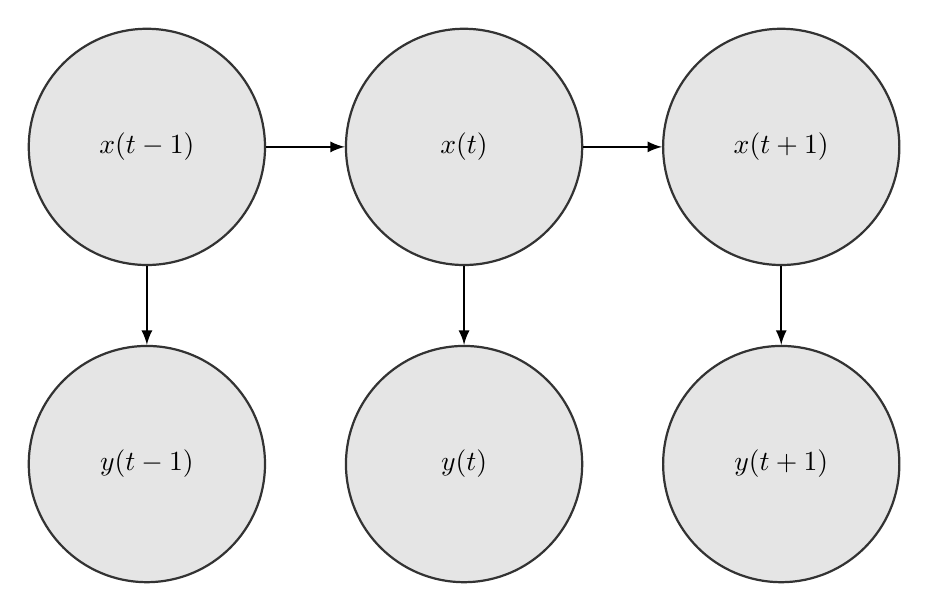
\begin{tikzpicture}
  \node[main,fill=black!10] (X1) {$x(t-1)$};
  \node[main,fill=black!10] (Xt) [right=of X1] {$x(t)$};
  \node[main,fill=black!10] (X2) [right=of Xt] {$x(t+1)$};
  \node[main,fill=black!10] (Y1) [below=of X1] {$y(t-1)$};
  \node[main,fill=black!10] (Yt) [below=of Xt] {$y(t)$};
  \node[main,fill=black!10] (Y2) [below=of X2] {$y(t+1)$};
  \path (X1) edge [connect] (Xt)
        (Xt) edge [connect] (X2);
  \path (X1) edge [connect] (Y1);
  \path (X2) edge [connect] (Y2);
  \path (Xt) edge [connect] (Yt);

\end{tikzpicture}
\end{center}

Вероятность увидеть последовательность \( Y=y(0), y(1),\dots,y(L-1) \) длины \( L \) равна

\[ P(Y)=\sum_{X}P(Y\mid X)P(X), \]

здесь сумма пробегает по всем возможным последовательностям скрытых узлов \( X=x(0), x(1), \dots, x(L-1). \) Метод подсчёта полным перебором значений \( P(Y) \) -- очень трудоёмкий для многих задач из реальной жизни в силу того, что количество возможных последовательностей скрытых узлов очень велико. Но применение процедуры прямого-обратного хода позволяет существенно увеличить скорость вычислений.

\subsubsection*{Условно-случайные поля}

Условные случайные поля -- дискриминативная ненаправленная вероятностная графическая модель, являющаяся разновидностью марковских случайных полей.

Метод УСП относится к дискриминативным вероятностным методам, в отличие от порождающих методов, таких как СММ или метод «Наивного Баеса».

При использовании дискриминативных моделей необходимо знать условное распределение \( P(T|X) \) на множестве значений скрытых переменных объекта Зная условное распределение мы можем определить наиболее вероятные значения скрытых переменных объекта. В отличие от порождающей модели, дискриминативная модель не позволяет моделировать новые объекты из генеральной совокупности. В случае, когда условная плотность неизвестна, ее можно попробовать настроить по обучающей выборке. Настройка дискриминативной модели более простая, поэтому если нам требуется только уметь определять значения скрытых переменных по наблюдаемым, использование такой модели предпочтительно.

В УСП выбор ключевых признаков для задания вероятности перехода между состояниями при наличии наблюдаемого значения зависит от специфики конкретных данных, но в отличие от СММ, УСП может учитывать любые особенности и взаимозависимости в исходных данных. Вектор признаков рассчитывается на основе обучающей выборки и определяет вес каждой потенциальной функции. Для обучения и применения модели используются алгоритмы, аналогичные алгоритмам СММ: Витерби и его разновидность – алгоритм «прямого-обратного» хода.

Наиболее распространенной в применении является модель линейных условно-случайных полей. Данная модель чаще всего применяется для решения задач разметки и сегментации последовательностей. УСП -- алгоритм машинного обучения с учителем.

Линейный УСП хорошо подходит для решения задач сегментации и разметки последовательности, например:
\begin{itemize}
\item автоматическое выделение ключевых слов из текстов;
\item автоматическое выделение (именованных) сущностей;
\item анализ тональности;
\item частеречное тэгирование;
\item автоматическое распознавание речи.
\end{itemize}

СММ можно рассматривать как частный случай линейного УСП.

Графовая модель СММ представлена на рисунке \_.

\begin{center}
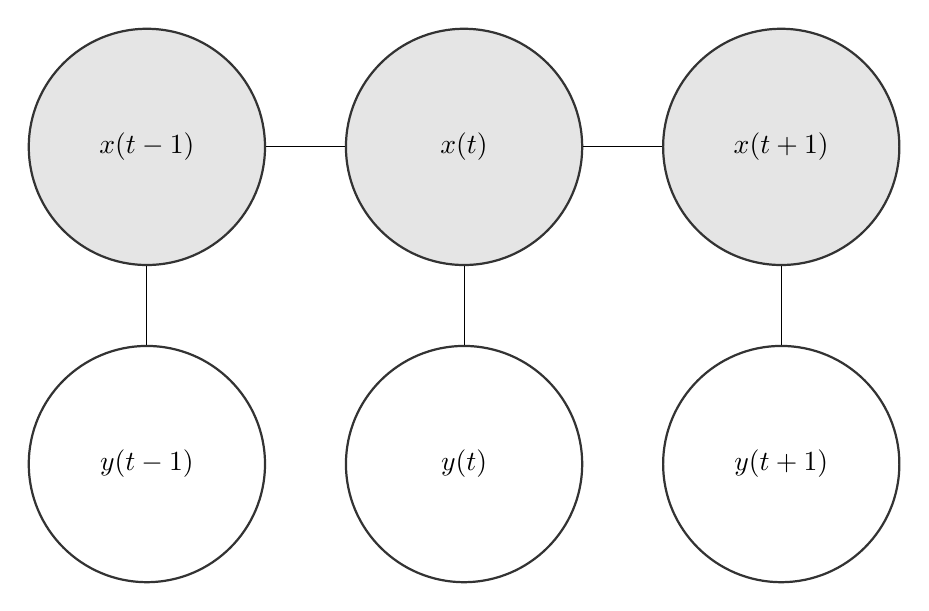
\begin{tikzpicture}
  \node[main,fill=black!10] (X1) {$x(t-1)$};
  \node[main,fill=black!10] (Xt) [right=of X1] {$x(t)$};
  \node[main,fill=black!10] (X2) [right=of Xt] {$x(t+1)$};
  \node[main] (Y1) [below=of X1] {$y(t-1)$};
  \node[main] (Yt) [below=of Xt] {$y(t)$};
  \node[main] (Y2) [below=of X2] {$y(t+1)$};
  \path (X1) edge node { } (Xt)
        (Xt) edge node { } (X2);
  \path (X1) edge node { } (Y1);
  \path (X2) edge node { } (Y2);
  \path (Xt) edge node { } (Yt);

\end{tikzpicture}
\end{center}

В условных случайных полях отсутствует т.н. label bias problem – ситуация, когда преимущество получают состояния с меньшим количеством переходов, так как строится единое распределение вероятностей и нормализация производится для всей модели, а не в рамках отдельного состояния. Это, безусловно, является преимуществом метода: алгоритм не требует предположения независимости наблюдаемых переменных. Кроме того, использование произвольных факторов позволяет описать различные признаки определяемых объектов, что снижает требования к полноте и объему обучающей выборки. В зависимости от решаемой задачи, на практике достаточно объема от нескольких тысяч до миллионов термов. При этом точность будет определяться не только объемом выборки, но и выбранными признаками.

Недостатком подхода УСП является вычислительная сложность анализа обучающей выборки, что затрудняет постоянное обновление модели при поступлении новых обучающих данных.

Сравнение метода УСП с некоторыми другими методами показывает, что предлагаемый метод работает лучше остальных (по мере F1) при решении различных лингвистических задач. Например, в задачах автоматического нахождения в тексте именованных сущностей УСП демонстрирует несколько меньшую точность по сравнению с методом СММ, но при этом значительно выигрывает в полноте.

На сегодняшний день именно метод УСП является наиболее популярным и точным способом извлечения объектов из текста.

\subsubsection*{Применение графовых моделей для классификации библиографических данных}
Графовые модели, представляющие собой модели переходов состояний, с разной степенью точности позволяют описывать библиографические записи, представляя каждый класс в качестве отдельного состояния. Опираясь на публикации последних лет [источники], можно сделать вывод, что метод условно-случайных полей является наиболее эффективным для классификации последовательностей на естественном языке, частным случаем которых являются библиографические данные. 

В то же время, классификация библиографических данных является самостоятельной задачей, для которой не годятся универсальные алгоритмы и их параметры для классификации последовательностей на естественном языке. Исследование и выявление признаков рассматриваемых классов, их функций и особенностей предобработки библиографических данных является важным шагом к разработке методики и алгоритма классификаций библиографических данных на основе модифицированного метода условно-случайных полей.

\section{Постановка целей и задач диссертационных исследований}

Современный прогресс вычислительной техники и информатики позволяет компьютеризировать рутинные задачи все большего числа предметных областей.
Одной из таких областей являются библиографические данные, обработка которых до сих пор представляет собой рутинный ручной труд оператора, подверженный влиянию человеческого фактора в виде ошибок и опечаток. Первым и важным шагов в решении данной проблемы является разработка алгоритмов классификации библиографических данных, необходимого для дальнейшего разбиения на структурные компоненты и преобразования к структурированным форматам, таким как XML и JSON.

В рамках достижения поставленной цели необходимо решить следующие задачи:
\begin{itemize}
\item в связи с развитием Интернета и увеличением потока информации, в современном обществе возникает потребность в компьютерном анализе и классификации данных, в том числе и библиографических данных. Библиографические данные, оформленные в соответствии со стандартами, представляют собой структурированную текстовую информацию, однако в общем случае и на практике они представляют собой слабо структурированную текстовую информацию. Аналитический обзор существующих программных продуктов показал, что обработка библиографических данных на русском языке является актуальной задачей;
\item важной составляющей классификации библиографических данных является выбор и модификация алгоритма машинного обучения, подбор признаков классов и их функций;
\item для определения и подтверждения качества и эффективности разработанных методики и алгоритма потребуется подбор и подготовка данных для тестирования, а также выбор и вычисление метрик в сравнении с другими методами классификации.
\end{itemize}

\section*{Выводы к главе 1}
\addcontentsline{toc}{section}{Выводы к главе 1}

Обзор российских и международных стандартов оформления библиографических данных позволил ознакомиться с формами информационного представления библиографических записей. В качестве основного стандарта оформления данных для классификации был выбран ГОСТ 7.0.5-2008, являющийся основным российским стандартом оформления библиографических записей.

Рассмотрение машиночитаемых стандартов представления библиографических данных позволило выделить ключевые структурные элементы библиографических записей для информационного обмена с помощью компьютера, что является необходимым для решении задачи структуризации библиографических данных в программных средствах.

Были выделены следующие ключевые структурные элементы: имена авторов, название публикации, название издания, местоположение и название издательства, номер тома или выпуска, год издания и диапазон страниц.

Аналитический обзор существующих программных средств классификации библиографических данных показал, что существующие решения обладают одним или несколькими из следующих принципиальных недостатков: ручной ввод структурных элементов библиографических записей для дальнейшего структурирования, требование к точному совпадению библиографических данных с определенным стандартом, плохая поддержка русского языка или полное ее отсутствие.

Аналитический обзор существующих методов классификации библиографических данных показал, что метод условно-случайных полей является наиболее эффективным для классификации последовательностей на естественном языке [источники], однако нуждается в доработках, необходимых для эффективной обработки библиографических данных в формате ГОСТ 5.0.7.-2008, в том числе анализе структурных элементов и выделении их функций признаков, предобработке и очистке данных перед работой выбранного метода.

Таким образом аналитический обзор современного состояния программных средств и методов классификации библиографических данных показал, что задача диссертации, заключающаяся в исследовании и разработке методики и алгоритма классификации библиографических данных с помощью условно-случайных полей, является актуальной и найдет свое применение в существующих и принципиально новых программных средствах.

\chapter{Разработка методики и алгоритма классификации библиографических данных с помощью условно-случайных полей}
Lorem ipsum dolor sit amet, consectetur adipiscing elit.

\section{Формализованное представление задачи классификации библиографических данных}
Lorem ipsum dolor sit amet, consectetur adipiscing elit.

\subsection{Логарифмические линейные модели}
Lorem ipsum dolor sit amet, consectetur adipiscing elit.

\subsection{Метод условно-случайных полей}
Lorem ipsum dolor sit amet, consectetur adipiscing elit.

\section{Разработка методики классификации библиографических данных}
Lorem ipsum dolor sit amet, consectetur adipiscing elit.

\subsection{Подбор данных для обучения модели}
Lorem ipsum dolor sit amet, consectetur adipiscing elit.

\subsection{Подготовка и нормализация данных}
Lorem ipsum dolor sit amet, consectetur adipiscing elit.

\subsection{Обучение модели}
Lorem ipsum dolor sit amet, consectetur adipiscing elit.

\subsection{Проверка адекватности обучения модели}
Lorem ipsum dolor sit amet, consectetur adipiscing elit.

\subsection{Использование модели}
Lorem ipsum dolor sit amet, consectetur adipiscing elit.

\section{Разработка алгоритма классификации библиографических данных}
Lorem ipsum dolor sit amet, consectetur adipiscing elit.

\subsection{Выбор структурных элементов и меток}
Lorem ipsum dolor sit amet, consectetur adipiscing elit.

\subsection{Выявление признаков структурных элементов библиографических данных}
Lorem ipsum dolor sit amet, consectetur adipiscing elit.

\subsection{Составление графовой модели}
Lorem ipsum dolor sit amet, consectetur adipiscing elit.

\subsection{Составление функций признаков}
Lorem ipsum dolor sit amet, consectetur adipiscing elit.

\section*{Выводы к главе 2}
\addcontentsline{toc}{section}{Выводы к главе 2}
Lorem ipsum dolor sit amet, consectetur adipiscing elit.

\chapter{Исследование и разработка методики и алгоритма обработки и структуризации библиографических данных}
Lorem ipsum dolor sit amet, consectetur adipiscing elit.

\section{Разработка обобщенной модели обработки и структуризации библиографических данных}
Lorem ipsum dolor sit amet, consectetur adipiscing elit.

\subsection{Выбор структурных элементов и меток}
Lorem ipsum dolor sit amet, consectetur adipiscing elit.

\subsection{Составление графовой модели}
Lorem ipsum dolor sit amet, consectetur adipiscing elit.

\section{Разработка методики и алгоритма обработки и структуризации библиографических данных}
Lorem ipsum dolor sit amet, consectetur adipiscing elit.

\subsection{Выявление признаков структурных элементов библиографических данных}
Lorem ipsum dolor sit amet, consectetur adipiscing elit.

\subsection{Составление функций признаков}
Lorem ipsum dolor sit amet, consectetur adipiscing elit.

\subsection{Предобработка данных}
Lorem ipsum dolor sit amet, consectetur adipiscing elit.

\section*{Выводы к главе 3}
\addcontentsline{toc}{section}{Выводы к главе 3}
Lorem ipsum dolor sit amet, consectetur adipiscing elit.


\backmatter %% Здесь заканчивается нумерованная часть документа

\include{40_outro}

\bibliographystyle{gost780u}
\bibliography{biblio}

\include{60_extra}

\end{document}
